% ERW / Libros Digitales — summary poster
% Single-page A3 portrait, compiles with pdflatex
\documentclass[11pt]{article}

\usepackage[a3paper, portrait, margin=1.4cm, top=1.0cm, bottom=1.0cm]{geometry}
\usepackage[T1]{fontenc}
\usepackage[utf8]{inputenc}
\usepackage{lmodern}
\usepackage{microtype}
\usepackage{graphicx}
\usepackage{xcolor}
\usepackage[most]{tcolorbox}
\usepackage{multicol}
\usepackage{enumitem}
\usepackage{amsmath, amssymb}
\usepackage[hidelinks]{hyperref}
\usepackage{tikz}
\usetikzlibrary{positioning, arrows.meta, shapes.geometric}

\graphicspath{{../paper/figures/}}

% Uninorte-ish palette
\definecolor{unBlue}{HTML}{003B71}
\definecolor{unGold}{HTML}{C8A028}
\definecolor{unLight}{HTML}{EAF1F8}
\definecolor{unGray}{HTML}{4A4A4A}

\tcbset{
  posterbox/.style={
    enhanced, colback=white, colframe=unBlue,
    boxrule=0.6pt, arc=2pt, left=6pt, right=6pt, top=4pt, bottom=4pt,
    fonttitle=\bfseries\color{white},
    coltitle=white, colbacktitle=unBlue,
    title=#1, attach boxed title to top left={xshift=4pt, yshift=-2pt},
    boxed title style={colback=unBlue, sharp corners, boxrule=0pt},
    before skip=6pt, after skip=6pt,
  }
}

\setlength{\columnsep}{0.6cm}
\setlength{\parindent}{0pt}
\setlength{\parskip}{2pt}
\pagestyle{empty}

% Compact list spacing
\setlist[itemize]{leftmargin=*, topsep=2pt, itemsep=1pt, parsep=0pt}

\begin{document}

% ===================== HEADER =====================
\begin{tcolorbox}[enhanced, colback=unBlue, colframe=unBlue, sharp corners,
                  left=10pt, right=10pt, top=8pt, bottom=8pt, boxrule=0pt]
  {\color{white}\bfseries\Huge Implementation of Shrinkage Estimators\\[2pt]
                              for Cosmological Precision Matrices\par}
  \vspace{6pt}
  {\color{white!90!black}\large
   \textbf{Andrés F. Movilla Obregón} \,\textperiodcentered\,
   \textit{amovilla1103@gmail.com}
   \hfill
   \textbf{Advisor:} Elias D.\ Niño-Ruiz, Ph.D.\,\textperiodcentered\,
   \textit{enino@uninorte.edu.co}\par}
  \vspace{2pt}
  {\color{unGold}\small
   M.Sc.\ in Systems and Computer Engineering \,\textperiodcentered\,
   Universidad del Norte \,\textperiodcentered\,
   Engineering Division\par}
\end{tcolorbox}

\vspace{2pt}

% ===================== TWO-COLUMN BODY =====================
\begin{multicols}{2}

% ---- Context / Introduction ----
\begin{tcolorbox}[posterbox=Context]
\small
Two very different problems share the same statistical bottleneck. In
\textbf{weather forecasting}, ensemble Kalman filters combine model predictions
with observations to keep forecasts on track. In \textbf{cosmology},
parameter inference from galaxy surveys turns measurements into estimates of
the universe's contents. Both rely on inverting a \emph{covariance matrix}
estimated from a small number of simulations or model runs.

When the matrix is built from too few samples, the inverse is unstable: tiny
noise in the inputs produces huge errors in the outputs. The result is poor
forecasts and unreliable cosmological parameters.

\textbf{Shrinkage estimators} address this by blending the noisy estimate
with a structured \emph{target}. The trick is choosing the right blend at
every step --- and choosing it well matters. In numerical weather
prediction, an unstable covariance translates into degraded forecasts;
in cosmological surveys, it translates into wider error bars on
fundamental parameters such as the dark-energy equation of state.

This work integrates a rigorous shrinkage framework into the
\emph{sequential} setting of the Ensemble Kalman Filter, where the
estimate is recomputed at every assimilation cycle, and asks a
practical question: \emph{which estimator should a practitioner pick,
and on what basis?}
\end{tcolorbox}

% ---- Objectives ----
\begin{tcolorbox}[posterbox=Objectives]
\small
\begin{itemize}
\item Embed the \emph{direct precision shrinkage} framework
      (Bodnar et al.) inside the dual formulation of the Ensemble
      Kalman Filter (EnKF), recomputing coefficients each cycle.
\item Implement and compare \textbf{six shrinkage estimators} plus two
      EnKF baselines on systems with opposite precision structure.
\item Propose a \textbf{scaled-identity target} that needs no
      domain-specific information.
\item Release all implementations in the open-source TEDA framework.
\end{itemize}
\end{tcolorbox}

% ---- Methodology ----
\begin{tcolorbox}[posterbox=Methodology]
\small
\textbf{The assimilation cycle.} At each step, an ensemble of states is
propagated by the model, mixed with new observations, and updated. The
covariance of the ensemble determines how observations are weighted.
\vspace{4pt}

\begin{center}
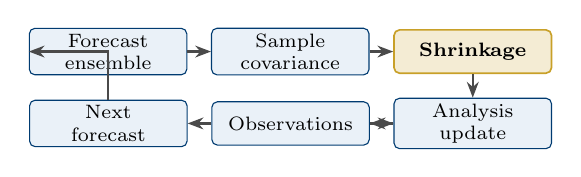
\begin{tikzpicture}[
  node distance=3mm and 3mm,
  every node/.style={font=\scriptsize},
  box/.style={draw=unBlue, fill=unLight, rounded corners=2pt,
              minimum width=2.0cm, minimum height=0.55cm, align=center,
              inner sep=2pt},
  hilite/.style={draw=unGold, fill=unGold!20, rounded corners=2pt,
                 minimum width=2.0cm, minimum height=0.55cm, align=center,
                 inner sep=2pt, line width=0.6pt},
  arr/.style={-{Stealth[length=2mm]}, unGray, thick}
]
\node[box] (fc)  {Forecast\\ ensemble};
\node[box, right=of fc] (cov) {Sample\\ covariance};
\node[hilite, right=of cov] (sh) {\textbf{Shrinkage}};
\node[box, below=of sh] (an) {Analysis\\ update};
\node[box, left=of an] (obs) {Observations};
\node[box, left=of obs] (next) {Next\\ forecast};

\draw[arr] (fc) -- (cov);
\draw[arr] (cov) -- (sh);
\draw[arr] (sh) -- (an);
\draw[arr] (obs) -- (an);
\draw[arr] (an) -- (obs);
\draw[arr] (obs) -- (next);
\draw[arr] (next.north) |- (fc.west);
\end{tikzpicture}
\end{center}

\textbf{Estimators evaluated.} Four \emph{direct precision} targets
(identity, scaled-identity \emph{[ours]}, eigenvalue, cosmological), one
\emph{covariance-space} method (Ledoit--Wolf), and the nonparametric
\emph{NERCOME}. Two baselines: standard EnKF and EnKF--Cholesky.

\begin{center}
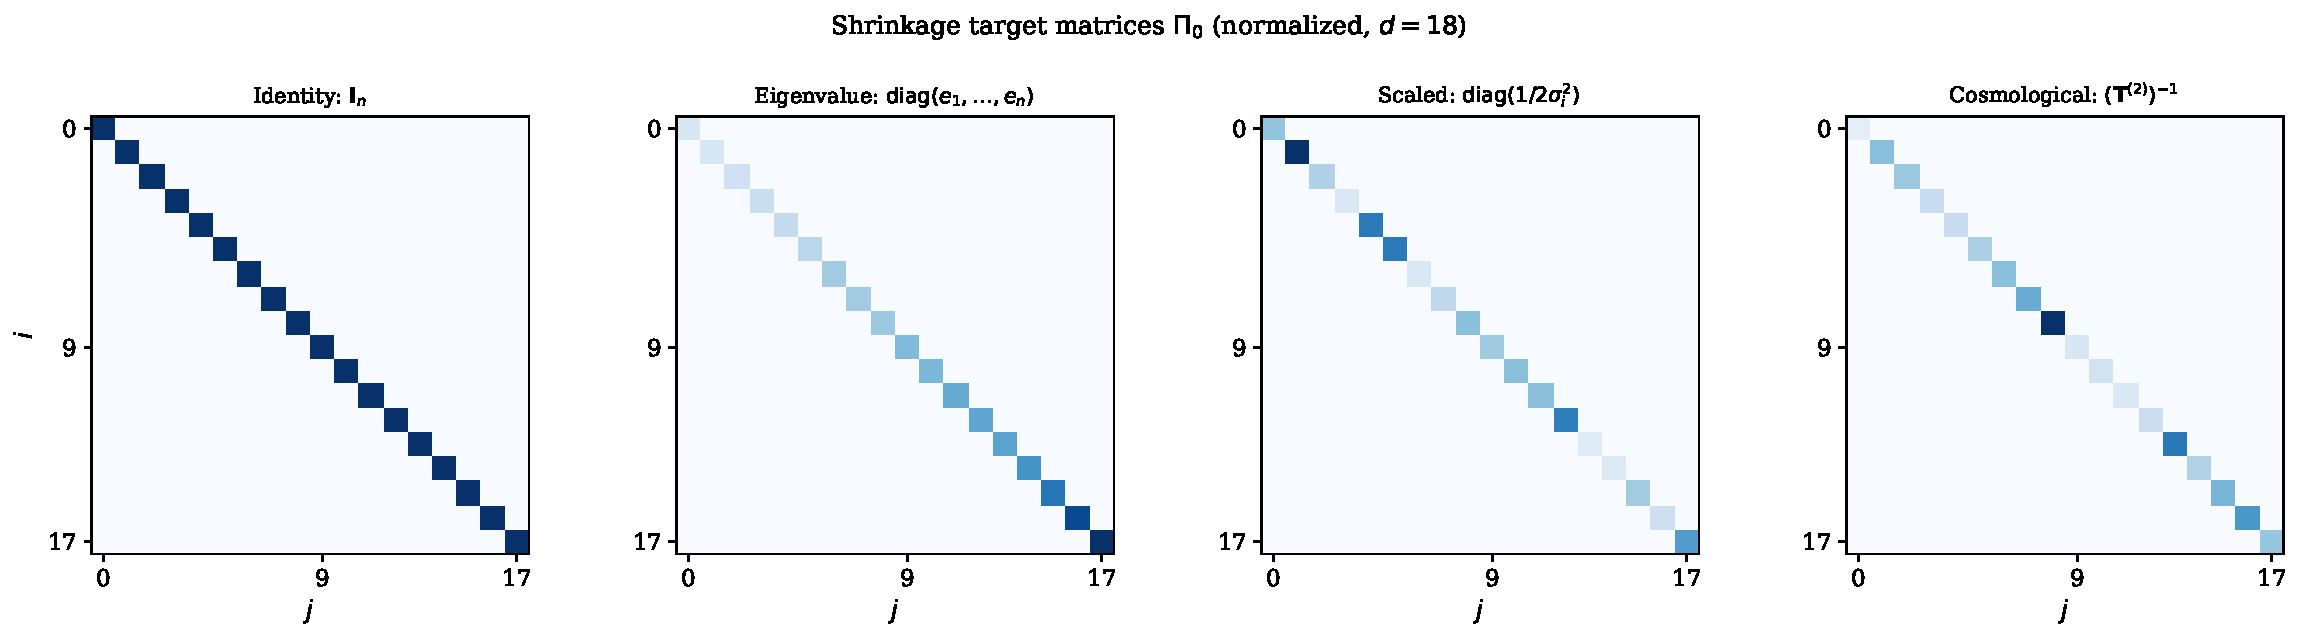
\includegraphics[width=0.92\linewidth]{target_comparison.pdf}\\[1pt]
{\footnotesize Shrinkage targets compared: structure imposed on the
estimate determines how the noisy sample is regularized.}
\end{center}

\textbf{Test systems.} Two systems with opposite precision structure
to stress-test target-truth alignment:
\begin{itemize}
\item \textbf{Lorenz~96} ($n{=}40$): chaotic atmospheric model with
      \emph{dense} off-diagonal precision from spatial coupling.
\item \textbf{BOSS DR12 mocks} ($d{=}18$): cosmological power-spectrum
      data with \emph{near-diagonal} precision from independent k-bins.
\end{itemize}

\begin{center}
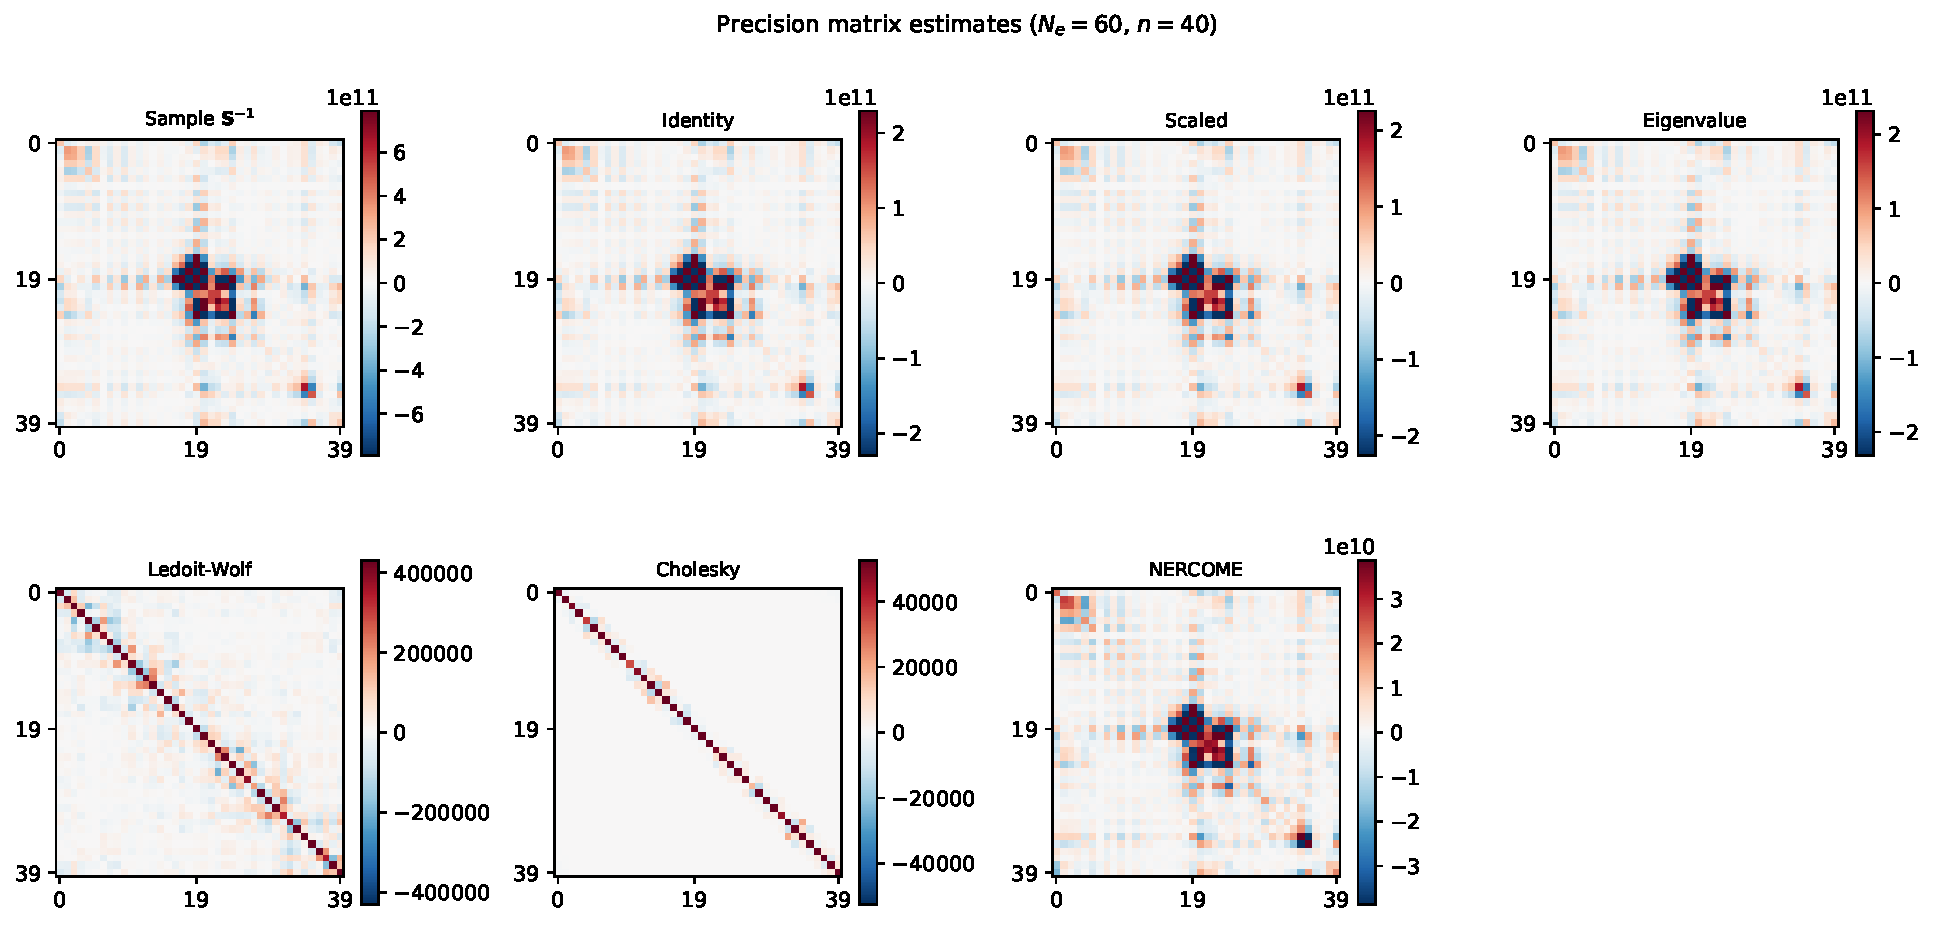
\includegraphics[width=0.92\linewidth]{precision_heatmap.pdf}\\[1pt]
{\footnotesize True precision matrices: Lorenz~96 (left, dense) vs.\
BOSS DR12 (right, near-diagonal).}
\end{center}
\end{tcolorbox}

% ---- Results ----
\begin{tcolorbox}[posterbox=Main Results]
\small
\textbf{Result 1 --- target alignment is decisive.} Diagonal targets break
on Lorenz~96 (dense precision) but excel on cosmological data
(near-diagonal precision).

\begin{center}
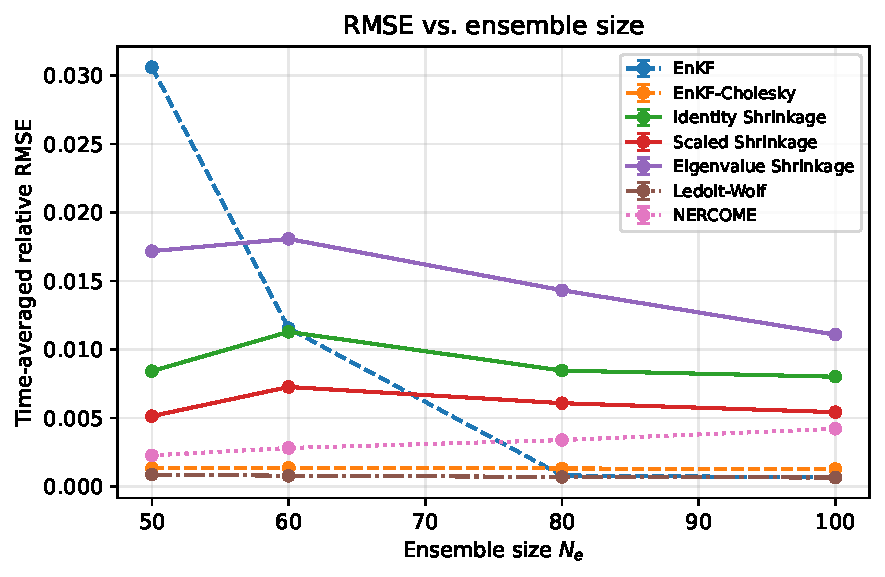
\includegraphics[width=0.96\linewidth]{rmse_vs_ne.pdf}\\[1pt]
{\footnotesize Lorenz~96: RMSE vs.\ ensemble size. Diagonal-target
shrinkage is unstable; Ledoit--Wolf is most stable.}
\end{center}

\vspace{2pt}
\textbf{Result 2 --- best estimator $\neq$ best filter.} On cosmological
data, Ledoit--Wolf produces the \emph{worst} standalone precision
estimates yet the \emph{lowest} EnKF RMSE. Low cycle-to-cycle variance
matters more than low bias.

\begin{center}
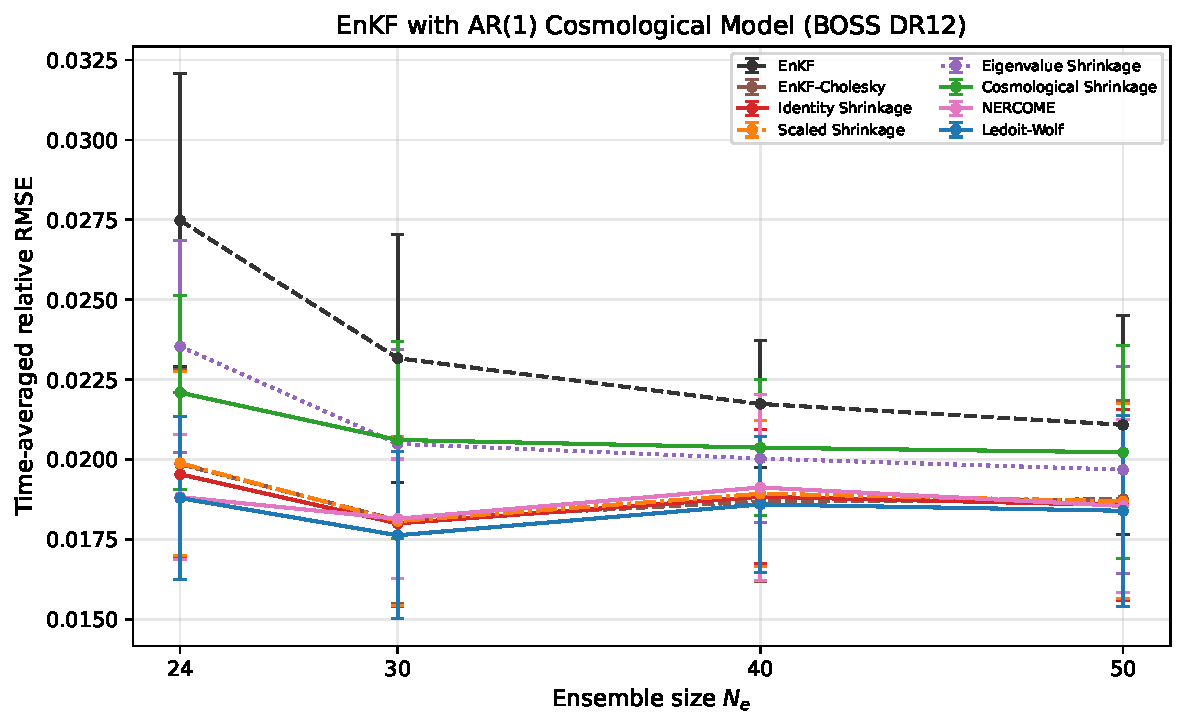
\includegraphics[width=0.96\linewidth]{cosmo_enkf_rmse.pdf}\\[1pt]
{\footnotesize Cosmological data: EnKF RMSE across estimators. The most
biased standalone estimator wins the sequential filter.}
\end{center}

\end{tcolorbox}

% ---- Key Numbers ----
\begin{tcolorbox}[posterbox=Key Numbers]
\small
\begin{itemize}
\item \textbf{6} shrinkage estimators \,\textperiodcentered\, \textbf{2} EnKF baselines
\item Misaligned targets: cond.\ \textbf{$10^7$--$10^{11}$}, $\beta^*$ up to \textbf{$10^9$}, clamping fires in \textbf{$>$80\%} of cycles
\item Scaled-identity target: \textbf{10--30\%} gain over plain identity
\item Ledoit--Wolf stdev across cycles: \textbf{$\pm 0.01$} vs.\ \textbf{$\pm 0.13$} for direct precision
\end{itemize}
\end{tcolorbox}

% ---- Conclusions ----
\begin{tcolorbox}[posterbox=Conclusions]
\small
\begin{itemize}
\item \textbf{Target-truth alignment} drives the success or failure of
      direct precision shrinkage; there is no one-size-fits-all target.
\item \textbf{Variance reduction beats bias reduction} for sequential
      filtering: standalone metrics like Frobenius loss can mislead
      practitioners choosing an estimator for the EnKF.
\item The proposed \textbf{scaled-identity target} gives a 10--30\%
      improvement over plain identity on both systems with no
      domain-specific tuning.
\item Practical impact: more reliable forecasts and cosmological
      parameter estimates from the same limited ensembles.
\end{itemize}
\end{tcolorbox}

% ---- Future Work ----
\begin{tcolorbox}[posterbox=Future Work]
\small
\begin{itemize}
\item Combine shrinkage with \textbf{spatial localization} for
      high-dimensional models (weather, $n{\sim}10^6$).
\item \textbf{Adaptive targets} that track the evolving precision
      structure across cycles.
\item Theoretical treatment of the \textbf{variance--bias trade-off} in
      sequential filtering (discrete Lyapunov framework).
\item Extension to \textbf{nonlinear, non-Gaussian} ensembles.
\end{itemize}
\end{tcolorbox}

% ---- Resources ----
\begin{tcolorbox}[posterbox=Resources]
\small
\textbf{Full thesis (PDF):}\\
{\footnotesize\url{https://github.com/andremov/TEDA/blob/main/thesis/main.pdf}}\\[2pt]
\textbf{Scientific paper, LNCS (PDF):}\\
{\footnotesize\url{https://github.com/andremov/TEDA/blob/main/paper/main.pdf}}\\[2pt]
\textbf{TEDA framework (code):}\\
{\footnotesize\url{https://github.com/andremov/TEDA}}
\end{tcolorbox}

\end{multicols}

\end{document}
